\chapter{State of the Art} \label{chap:state-of-the-art}
In this section we will discuss the current state of the art in game development with a programming perspective.

Before we begin explaining the \ac{SotA} it is important to note that there are two types of game programming. The first one will be referred to as \textit{\dquote{Engine}} programming, which deals with tasks such as I/O, rendering and simulation \cite{blow2004game}. The other type is \textit{\dquote{Gameplay}} programming. Gameplay programming is used to define the rules and behaviour of the gameplay itself \cite{blow2004game}. In Unity3D the gameplay programming language is C\# and in Unreal it is C++. Other examples of gameplay languages exist, such as Lua \cite{lua:about,gamedev:lua} and GDScript for the Godot engine \cite{godot:gdscript}. Both of these types of development will be explored in greater detail later in this chapter (see \secref{gameplay:programming} and \secref{engine:programming}). The most common language in this category is C++. Sometimes these language types are interleaved, some places these are strictly separated.

Many engine programmers make extensive use of \textit{\dquote{Meta}} programming. Game engines often support a number of platforms \cite{BinSubaih2007ASO}. Therefore certain platform-specific retooling is necessary when building the engine. This is achieved using macros, in C and C++, or another kind of meta programming. Meta programming changes the content of the source code based on some parameters that can be set at build time, thus platform-specific code can be injected only when building for that platform.

When application code and core code is made to have a clear separation, like between the gameplay code and engine code, it is a data-driven architecture, which game development makes extensive use of. Data-driven development is an architecture in which you divide core component code from application code. So the core would be the game engine, and the application would be the different games that is made. In general this gives some advantages, like being able to have more reusable code, having a core system that rarely change and when it does, it is between applications. It also gives better abstraction level, having a clear division between what is application logic, and what is the core code base.

Data-driven development has not always been used in game development, as \figureref{game-dev-history} shows, there has been quite some change. In the early days of game development, games were hardwired into circuits, this was done around the 1940s all the way up to the 1970s \cite{cathod-hardwire}. These games had quite simple game logic. With the advancements in computer technology, game development moved from implementing games in wires to building hard coded games, where the engine and gameplay code was not separated. This change made games easier to modify than the ones implemented in hardware \cite{graetz1981origin}. These games were also often of simple game logic, and had to bypass operating systems, to get added speed. Later came game-independent game engines, these were introduced because of the increase in development cost, they made it possible to reuse code, making it possible to make multiple games in the same engine.

Games also became more complex, as more specialised components were introduced, such as Artificial Intelligence and Physics \cite{sherrod2006ultimate}.  One of the bigger issues with this model is that games are dependent on game engines. The reason for this is that the games make use of specific components that are provided by the game engine. There has been research into the possibility of developing games independent of game engines, such that games can easily can be ported between game engines, as described in \cite{BinSubaih2007ASO}. This can improve the use of multiple game engines, such that the focus is on the game logic creation and a game engine is just a package of specific libraries that can be used, depending on the target platform for the game. Some of the concerns with this idea is the performance and implementation overhead that the generality may incur \cite{BinSubaih2007ASO}. 

\begin{figure}[H]
    \centering
    \includegraphics[width=.8\textwidth]{images/Game-development/Game-dev-history.png} 
    \caption{A overview of the evolution of game development \cite{BinSubaih2007ASO}.}
    \label{fig:game-dev-history}
\end{figure}

\section{Game Development} \label{sec:game-development}
As the complexity of games rose, game engines became more widely used \cite{blow2004game}. A game engine's goal is to reduce development time by enabling a collaborative process between programmers and artists, such that they can work together in one environment, to produce an application.
In \cite{Anderson:2008:CRG:1496984.1497031} the authors state that research, into engine development and architectures, is lacking. Another paper by the same author provides a good overview of what a game engine architecture, with a scripting system (see \figureref{typical-architecture}) may look like \cite{5962102}. Game engines commonly include the core subsystems seen in \figureref{engine-subsystes}.

\begin{figure}[H]
    \begin{subfigure}[b]{\textwidth}
        \includegraphics[width=\textwidth]{images/Game-development/Typical-game-engine.png}
        \caption{Typical game engine architecture with components \cite{5962102}.}
        \label{fig:typical-architecture}
    \end{subfigure}
    \begin{subfigure}[b]{\textwidth}
        \includegraphics[width=\textwidth]{images/blow-complexity.png}
        \caption{Engine Code Complexity \cite{blow2004game}.}
        \label{fig:engine-compl}
    \end{subfigure}
    \caption{Game Engines, Theory and Practice.}
    \label{fig:engine-theo-prac}
\end{figure}

As game engines grew more complex, so did the subsystems of the engines \cite{blow2004game, nystrom2014game} (see \figureref{engine-compl}). Many of them are self-explanatory but the \textit{Core} system, of the engine, is a bit abstract. It is responsible for handling communication between the subsystems and ensuring correctness. It deals with memory management, file \ac{I/O} as well as handling startup of the game and all the associated devices \cite{nilson2007game}. 

\begin{figure}[H]
    \centering
    \begin{tasks}[style=itemize, column-sep=0mm, label-align=left, label-offset={0mm}, label-width={10mm}, item-indent={3mm}](3)%
        \task Audio
        \task Input
        \task Physics 
        \task Renderer
        \task Core
        \task Scripting
        \task Networking
        \task Artificial Intelligence
    \end{tasks}
    \caption{Engine Subsystems.}
    \label{fig:engine-subsystes}
\end{figure}

To showcase engine architecture, we will use the JOT engine as an example because it is an academic open source engine. JOT and its architecture is presented in \cite{amador2014jot}. JOT is a specialised modular multipurpose massively multiplayer online game engine \cite{amador2014jot}. The developers behind JOT had an interesting approach documenting their progress. The paper gave a design for JOT and specified the architecture, the whole project was for academic purposes.

JOT was implemented in Java, due to Java's multiplatform nature and the availability of third party applications and libraries. They also argue that there are already game engines, both for teaching and open source written in Java, so there would be a level of familiarity to the field. When looking at the JOT architecture (\figureref{Jot_layers}) it gives a clearer picture of each component needed, compared to that presented in \cite{5962102} (see \figureref{typical-architecture}). The figure defines what they make use of in their different components.

\subsubsection{Comparison}
Here we take a quick look at how JOT compares to the engine architecture from \cite{5962102} and the MMOG ecosystem put forward by \cite{blow2004game}.
We do this to see if game engines are constructed as described in the literature.

JOT provides many of the larger modules as displayed in \figureref{engine-compl}, although in larger modules. Note that the figure represents more than just the game engine, it's the whole system for a MMOG.
As it includes things such as persistent storage, separate client and servers, account registration, etc, it is not directly comparable with JOT.
It should however be possible to create both the game client and server with JOT, either by using the included modules or adding new ones.

There is some difference in the sub-division of modules between JOT and the engine architecture from \cite{5962102}. But in the coarse perspective they are similar. One way to attempt at fitting JOT into the model is the following (Engine architecture in bold, JOT in normal font): 
\begin{description} 
    \item[Engine Core] $\longleftrightarrow$ Infrastructure layer
    \item[Engine Modules] $\longleftrightarrow$ Modules from Core, (most of) Framework and Toolkit
    \item[Application specific code] $\longleftrightarrow$ Code that is above the framework layer in JOT
    \item[Resource Manager] $\longleftrightarrow$ (Part of) Managers from Framework layer
    \item[Game assets] $\longleftrightarrow$ Game assets
\end{description}

JOT is coarsely similar to the architecture and ecosystem presented by \cite{5962102} and \cite{blow2004game} respectively. There are minor differences in where components such as Physics and Rendering are placed, but overall they are similar.

\begin{figure}[H]
    \centering
    \includegraphics[scale = 0.6]{images/Game-development/Jot-layers.png}
    \caption{JOT architecture in layers \cite{amador2014jot}.}
    \label{fig:Jot_layers}
\end{figure}

When examining the core systems of a game engine, the programming language(s) is of particular interest in this project. The following section will examine scripting languages and what language(s) the game engine is implemented in.

\subsection{Gameplay Programming} \label{sec:gameplay:programming}
Gameplay programming often come in the form of scripting languages or \dquote{glue languages}. These are high-level languages used to develop game logic. They are one of the tools considered to be most important in modern game engines \cite{gamasutra:EngineSurvey, 5962102}. According to \cite{5962102} there is no clear definition of what a scripting language is, but they are generally used to control behaviour of other components. They often sacrifice run-time performance, in favour of writability. They often act as a layer of abstraction over subordinate components or programs \cite{5962102}.

Scripting systems make up a comprehensive list of applications and can be used in many different domains, depending on the application. Everything from command-line interpreters related to UNIX shells such as Ksh \cite{korn1994ksh}, to integrated scripting systems such as MEL(Maya Embedded Language) \cite{gould2003complete}, which for instance can be used to animate models in the Maya 3D graphics application.

Embedded scripting languages are often implemented for non-programmers \cite{gamedev:lua}. This is useful in game development, where a scripting system can be embedded in the computer game, which can be used to issue commands to the game engine such as loading objects, textures and levels, but also be used for more complicated tasks like playing an animated cut-scene or triggering events inside the game world. 
%A scripting language can also be embedded into the game engine, and give multiple uses.

According to \cite{5962102} the term scripting language is fuzzy and the authors propose a classification for scripting systems. This classification group script by what they are capable of solving. The categories are \cite{5962102}:
\begin{description}
    \item[Initialisation] are executed once during a program's run time, usually at the start. They are mostly used to set internal program parameters to the values given in the script.
    \item[Trigger-only] are split into event handler scripts and event oriented scripts. Both subcategories are used to execute scripts when a specific event happens in the game. \textbf{Event handler} scripts use events that are built into the game engine and define conditions on when to react to and what to do when a certain event occurs. \textbf{Event oriented} scripts are a bit more complicated. In these languages, the programmer defines triggers and conditions on when to react to certain events. Once every cycle the conditions are check and the appropriate triggers are invoked in case the conditions are met.
    \item[Program-like] defines two sub-categories; looping and regular scripts. Looping scripts are scripts that repeatedly execute, such that they keep reevaluating the current situation in the game. This means when the end of the script is reached, they restart execution from the beginning of the script. Regular scripts are scripts that execute once only. They will run from start to finish concurrently\footnote{It is not specified further in the source whether this is concurrency on multiple cores or thread-of-control} with the host application. But repeating operations, like loops, can be executed by the script.
\end{description}

\subsection{Engine Programming} \label{sec:engine:programming}
Industry game engines are often implemented in C++. The common belief with game developers is that C++ is a low-level, memory efficient language, used to get as much performance out of the hardware as possible\cite{gamasutra:c++functional}. According to Wikipedia C++ is used in many AAA studios and their engines, such as Unreal Engine 4 \cite{EpicGamesRepo}, Amazon Lumberyard \cite{awsRepo}, Unity3D \cite{wiki:Unity3D} and Frostbite \cite{wiki:Frostbite}.

Another language often used for open source and teaching material for game engine development is Java\cite{Java:Gamedev-tutorials}. It is of interest due to its multiplatform abilities, capabilities for multithreading and sockets\cite{amador2014jot}. Multithreading is important as \acp{CPU} no longer increase in clock frequency, but instead see an increase in the number of processing units, so it will lead to better utilisation of the \ac{CPU}\cite{Pfeffer2004}. Sockets provide a means for building multiplayer games \cite{freelancer:EngineLanguages}.

As an example, the original Minecraft game is implemented in Java. There also exist a C++ version, which was implemented by Microsoft after they bought the game \cite{pcgamersn:Minecraftinc++}. The general consensus in game development is that Java is not as favourable for game engine development as the garbage collector hinders performance, which is why it isn't used in big AAA game development \cite{gamasutra:MemoryHandling,youtubeJonathanBlow}.

%\subsection{Discussion}
%As we can see from our research\todo{not sure research is the right word} in game development as a field it is both very innovative\needcite, always using the newest technologies, adding new things on top of their game engine, to make games\todo[inline]{Bent skriver at dette ikke er tydeligt fra afsnittet. Jeg ved heller ikke personligt om jeg synes at vi har vist at noget er "innovativt"}. 
%But also very bound by tradition\footnote{Tradition here means the historical development process and tools of the industry.} and "what works". Why is it that game development is so obsessed with C++, and believe it is the most suited language for game engines.

%When they are so innovative and accepting of other technologies. Such as innovating new ways to make input to games, via new controllers, e.g. Wiimote or new modules such as \ac{VR} support to add complexity and new ways to give the user a fun gaming experience. At the foundation, game development uses C++ to make the underlying architecture, using arguments such as, they need as much performance as possible for their game engine\needcite.
%That they can't do what they do in C++, in other languages \cite{gamasutra:c++functional}.

%So they build these very effective game engines, pressing as much performance out of the hardware as possible, to then just put a scripting system on top, that is less effective and more sloppy with the use of memory\needcite.
%\todo[inline]{Bent skriver at det lyder populærvidenskabeligt, se forslag i kommentar.}

%Reasons why they are so stubborn using C++ may be that it is an industry that need to pump out as many games as possible to make a profit. So learning new technologies for their underlying systems might not be a priority when they can find good C++ programmers\todo{Excellent point, do we have a source?}.

%It might be that they think there is nothing better. Game development isn't a academic field, it is an industry. So reading the newest articles on development in language performance might not be relevant.
%So they are stuck thinking that C++ is the only language that can give them the performance they need\todo{This is conjecture}.
\section{Functional Programming} \label{sec:functional-programming} \todo{Is this better?}
In this section functional programming and it's central concepts are explored. An important distinction to keep in mind is the difference between a functional programming language and the discipline of functional programming. Functional programming languages such as, Haskell, Scheme or Standard ML are languages developed specifically for functional programming (the discipline). The discipline, however, is a paradigmatic methodology \cite{benton2016improving}.

Multi-paradigm programming languages such as C\#, Java or JavaScript support functional programming. The distinguishing features of functional programming are \cite{hudak1989conception}:
\begin{itemize}
    \item Higher order functions
    \item Lazy evaluation (Non-strict semantics)
    \item Data abstraction
    \item Equations and pattern matching
\end{itemize}

However, functional languages are made up of more components that provide additional expressive power and support. Some of these linguistic features are explained in the following sections.

\subsection{Higher Order Functions}
In the programming language C, functions cannot directly be passed as arguments to other functions\footnote{In C you can make a pointer to a function and pass that to a function.}. This means that functions are not first class. First-class functions is a linguistic feature that eases the use of higher order functions, which are functions that operate on other functions.

However, this feature can be useful in functional, as well as general, programming. Such functions are called higher order functions if they meet all of the following conditions:
\begin{itemize}
    \item Can be stored in a data structure
    \item Can be passed as arguments
    \item Can be returned as a result
\end{itemize}
Higher order functions can facilitate greater code reuse and modularity via function composition \cite{hughes1989functional}. An example of this is the general case function \ttt{map}, which takes a collection and a function. The function is then applied across the entire collection. This means that the supplied function is called once for each element of the collection, with the element as argument. The returned value is a collection of the return values from each of the functions calls.

\begin{lstlisting}[language=haskell, caption={Higher Order Functions in Haskell}, label={lst:haskell-map}]
    list = [1, 2, 3, 4, 5]
    increment n = n + 1
    
    map increment list
\end{lstlisting}

An example of \ttt{map} implemented in Haskell can be seen in \lstref{haskell-map}. The first line defines a list of five numbers, which is supplied to \ttt{map} on line 4. In addition to the list a function is has to be passed, which will be called by \ttt{map}. This function is defined on line two and it takes a number and increments it. The result of the map call on line 4 is \ttt{[2, 3, 4, 5, 6]}.

\subsection{Lazy Evaluation (Non-strict semantics)}
Non-strict semantics or lazy evaluation is an evaluation strategy. Programming languages such as C use eager evaluation, which means that commands are executed immediately and therefore evaluation order becomes the responsibility of the programmer. The advantage of lazy evaluation is that evaluation order is no longer the responsibility of the programmer. This allows for computation using infinite lists \cite{hudak1989conception}. Some of the advantages include:
\begin{itemize}
    \item Freeing the programmer from concerns about evaluation order
    \item Allowing for computation with unbounded infinite lists
\end{itemize}

Freeing the programmer from handling evaluation order means that evaluation can be postponed until it is absolutely necessary \cite{hudak1989conception}. This means that unused function calls written in the program, which are not need at runtime, are not called.

This enables the language to manage infinite lists in practice. Consider a list of all prime numbers, the list is not stored in memory, but rather calculated as necessary. Such a list is called a stream. If a stream is implemented in a language without lazy evaluation, the program would never finish calculating it, but due to lazy evaluation only the necessary elements are computed \cite{hughes1989functional}.

This very property results in a side effect. Lazy evaluation may prevent a thread from returning anything useful. This is because lazy evaluation means that results are only returned if they are needed and this need is difficult to translate across threads \cite{trinder1998algorithm+}. Therefore, in languages with lazy evaluation, parallelism is usually handled using eager evaluation \cite{o2008real}. \btc{Kunne måske udvides med noget om lazy eval in C\# using yield return ..}

\subsection{Monads}
Monads can be described as a design pattern for types \cite{lippert-blog:monad}. The pattern is used to encapsulate code such as functions, inputs, outputs and other operations. Monads come from category theory \cite{mac2013categories}, but are also used in functional programming. Monads are formally defined by a Kleisli triple, which consists of the following \cite{wadler1992essence}:
\begin{center}
\begin{tabular}{l l}
    A type constructor & \ttt{M t} \\
    A unit function & \ttt{t $\rightarrow$ M t} \\
    A binding operation & \ttt{M t $\rightarrow$ (t $\rightarrow$ M u) $\rightarrow$ M u}
\end{tabular}    
\end{center}
The type constructor defines how to obtain the type of the monad. In Haskell, if \ttt{M} is the monadic type and \ttt{t} is the data type, then the type constructor is \ttt{M t}. The unit function injects a value in the data type into the monadic type. In Haskell: \ttt{t $\rightarrow$ M t}. Finally the binding operation is a function with the type \ttt{M t $\rightarrow$ (t $\rightarrow$ M u) $\rightarrow$ M u}. This function takes a monadic type and binds it to another monadic type. This is achieved by using the type constructor of the first monad and the unit function of the second monad. This results in a monad of the second type.

In order to ensure monad behaviour, it is restricted by the monad laws \cite{haskell-wiki:monad-laws}:
\begin{enumerate}
{\footnotesize
    \item \ttt{\textbf{do} { x <- return v; f x } $\equiv$ \textbf{do} { f v }}
    \item \ttt{\textbf{do} { x <- m; return x } $\equiv$ \textbf{do} { m }}
    \item \ttt{\textbf{do} { y <- \textbf{do} { x <- m; f x }; g y } $\equiv$ \textbf{do} { x <- m; y <- f x; g y }}
}
\end{enumerate}

These laws ensure that the monad behaves in accordance with the Kleisli triple. \btc{Hvad skal I bruge dette afsnit til?}

\subsection{Pure Functions \& Immutability}
In functional programming, functions are divided into two classes: pure and impure. In some cases, such as Haskell, impure functions are disallowed, however many functional languages allow impure functions. In imperative languages impure functions are commonly used. The definition of a pure functions is the following:

\quoteWithCite{A pure function is a function that, given the same input, will always return the same output and does not have any observable side effect.}{Professor Frisby}{frisby-mostly-adequate:guide-to-functional-programming} 

The main argument for disallowing impure functions is that reliance on state contributes to system complexity. \cite{moseley2006out}. Another important aspect is that pure functions are easily parallelised because they do not depend on external factors \cite{milewski:pure-functions-laziness-io-monads}. This further means that the order of function evaluation does not matter.

In order to limit or in some cases (Haskell) disallow mutability, functional programming languages restrict assignment. In the Scheme programming language assignment is available but uses special syntax to signify the impure action. In most cases where assignment would have occurred in an equivalent imperative language, functional languages use binding instead \cite{milewski:pure-functions-laziness-io-monads}. The difference between assignment and binding is that binding does not place data in a memory cell with an alias, but rather associates some data with a name. A binding cannot be changed once it has been made.

\subsection{List Comprehensions and Streams}
List comprehension is a list building notation used in several languages. It is based on set builder notation from set theory \cite{rosen2011discrete}. The notation is used in mathematics, \acp{GPL}, imperative as well as functional programming languages. However, functional languages can utilise this concept to create infinite lists or streams, of arbitrary content.

A number of languages, such as C\#, have implemented list comprehensions or similar constructs. \btc{nogle kode eksempler ville måske være godt}
\section{Meta-Programming} \label{sec:meta-programming} 
Meta programming is a programming technique in which programs have the ability to treat programs as data. Meta programming can be used to move computation from run-time to compile-time, to generate code using compile time computations, and to enable self-modifying code \cite{chlipala2010ur} \cite{czarnecki2000generative}. This can be useful in game engines as well, therefore we looked into their use in game development.

Our research failed to find any literature on on the subject, therefore in order to examine the use of macros we initially examined Unreal Engine. We chose this engine because it's popular, open source and written in C++. However, we decided to examine more open source game engines, three in total: Epic Games' Unreal Engine\footnote{Unreal Engine Github repository: \url{https://github.com/EpicGames/UnrealEngine}}, Godot\footnote{Godot Github repository: \url{http://google.com}} and Amazon's Lumberyard\footnote{Lumberyard Github repository: \url{http://google.com}}.

In each of the three Github repositories, we isolated the engine code (all three come with an editor as well). We wrote a small program in C\# that searches for all files with the extensions .c, .cpp, .h or .hpp. In these files we counted the number of \ttt{\#define}s, \ttt{\#ifdef}s and \ttt{\#if}s. The program is listed in \appendixref{unreal:macros}

\tableref{macros:in:ges} lists the number of lines of source code in each engine along with the number of macros. These results indicate that macros are in fact being used in game engine development (though not broadly applicable due to the limited data set).

\makeTable{{|l|c|c|c|c|}
    \hline
    \textbf{Engine} & \textbf{LoC} & \textbf{\ttt{\#define}s} & \textbf{\ttt{\#ifdef}s} & \textbf{\ttt{\#if}s}  \\
    Unreal Engine   & 15,027,722    & 350,300 & 51,945  & 171,914 \\
    Godot           & 1,590,009     & 25,809  & 6323    & 18,285 \\
    Lumberyard      & 2,345,289     & 28,885  & 3360    & 16,403 \\
    \hline}{Macro usage in open source game engines}{macros:in:ges}

Meta-programming can move computations from compile-time to run-time, which for instance may be used to do run-time code generation. Meta-programs can be anything from compilers, interpreters, type checkers, theorem provers, program generators, transformation systems, and program analysers.

In all of these cases, the meta-program manipulates a data object that represents the program itself \cite{sheard2001accomplishments}. When talking about types of meta-programs, there are two sub categories, program generators and program analysers\cite{pasalic2004role}. A program generator solves problems by generating a program that solves a particular instance of the problem. Usually the generated program is "specialised" for a particular problem instance and uses less resources than a general purpose, non-generated solution \cite{sheard2001accomplishments}.

Program analysers observe the structure, environment and program thereafter it computes some values as a result.  These results can be data- or control-flow graphs, or even another program with properties based on the properties of the source program\cite{sheard2001accomplishments}. In addition to these kinds of meta-programs as generators and analysers, or a mixture of both, there are several other distinctions; static vs run-time, manually vs automated annotated and homogeneous vs heterogeneous.

Program generators can come in two variants. Static generators generate code which is written to disk and later processed with normal compilers\cite{czarnecki2002generative}. Run-time code generators are programs that write or construct other programs, and then immediately execute the programs they have generated. The core of program generators is partitioned into static and dynamic code fragments\cite{sztipanovits2002generative}. The static code is the meta-program and the dynamic comprises the object-program, the program being produced. Staging annotations can be used to separate these two pieces\cite{sztipanovits2002generative}. If developers place the staging annotations directly themselves in the meta-programming system, then it is called a manual-staging system. On the other hand, if the staging annotations are placed by an automatic process, then the meta-programming system is called an automatic-staged system\cite{sztipanovits2002generative}.

There are two other very distinct types of meta-programming systems: homogeneous and heterogeneous systems. 
Homogeneous systems are systems where both the meta program and the object program share the same language, and heterogeneous systems where the meta-language is different from the object-language\cite{sheard2001accomplishments}.

\subsection{Meta-Programming Uses}
Meta-programming provides various benefits to users. Some of the these benefits are: performance, partial evaluation, translation, reasoning and mobile code.

\begin{description}
    \item[\textbf{Performance}]
    Meta-programming provides mechanisms allowing general purpose programs to be written as interpretive programs while maintaining performance; without the usual interpretive overhead \cite{sheard2001accomplishments}. An example of such a system is the Mix evaluator \cite{jones1989mix}.

    \item[\textbf{Partial Evaluation}] 
    Partial evaluation is another meta-programming technique to improve performance. The goal is to find and perform as many calculations before run-time as possible. These values are replaced by literals in the compiled code.

    \item[\textbf{Translation}]
    Translating one object-program to another object-program. The source and target language might be the same, but it not required. Examples of translators are compilers and program transformation systems\cite{sheard2001accomplishments}.

    \item[\textbf{Reasoning}]
    Meta-programming allows developers to reason about a object-program. If an object-program is written in a formal language, an analysis can discover properties of the object-program. These properties can be used to improve performance, provide assurance about the object-program behaviour, or validate meaning preserving transformations. Examples of reason meta-programs can be analysis such as flow analysis and type checkers.

    \item[\textbf{Mobile code}]
    Recently meta-programming has been used as a means for program transportation. Instead of using networks to bring data to programs, networks are used to bring the program to the data. Due to security concerns, intentional representations of programs are transported across the network\cite{Hornof:1999:CCR:609149.609203},\cite{Thibault:1998:SEA:829523.830979}. These representations can be formally verified that they do not compromise the integrity of the host machines they run on. The transported programs are object-programs\footnote{Object programs can be represented in various formats including text and intermediary formats such as Java Byte code.} and the analysers are meta-programs.
\end{description}

The reason meta-programming systems are useful, is because they make manipulation of objects and object-programs easier. It can be easy to use and understand by the programmer, provide high-level abstraction that captures the details of both the object-language and the patterns used by the meta-program\cite{sheard2001accomplishments}.





\section{Staged Programming}
In this section staged programming is discussed. Some staged programming technologies are also explored. These techniques are used in John Blow's programming language project: Jai \cite{youtubeJonathanBlow}. The idea is that some computation can be moved to compile time as well as generating platform-specific code. In Jai any function can be called at compile-time \cite{github:jaiPrimer}, thus achieving staged programming without macros.

Staged programming comes in many forms ranging from C++ Templates\footnote{Note that while C++ Templates, are meta programming, they are technically not staged programming. But we believe that they make a good example anyway.} \cite{c++:templates} to MetaML \cite{sheard1998using}. Other initiatives have also attempted to implement staged programming in other languages, such as Haskell \cite{sheard2002template}.

The goal of staged programming is to create languages that provide constructs that efficiently and concisely express common functionality and impose little to no overhead in computation time. There are also other approaches that pursue similar goals, such as Scrap Your Boilerplate \cite{lammel2003scrap} or Lightweight Modular Staging \cite{rompf2010lightweight}.

\subsection{C++ Templates}
C++ Templates allow the programmer to implement functions that operate on generic parameters, i.e. write functions that work on a broad range of different parameters \cite{c++:templates:tutorial}. Though not always classified as staged programming, it still has the same flavour and will suffice in this discussion.
\lstref{c++:max:template} shows an implementation of a \ttt{Max}-template, which returns the greater of two arguments. This template can operate on any types where the greater than operator (\textgreater) is implemented. In this concrete example, the template accepts two arguments of the same generic type. If the programmer wishes to implement a template with two or more different generic types, he/she would need to add the types to the template constructor (\ttt{template \textless class T, class U\textgreater} for a template with two generic types).

\begin{lstlisting}[label={lst:c++:max:template}, caption={\ttt{Max}-function template in C++}]
template <class T>
T Max (T a, T b) {
  T result;
  result = a > b  ? a : b;
  return (result);
}
\end{lstlisting}

When a template is instantiated in the surrounding code (for instance \ttt{Max\textless int\textgreater (10, 20)}), the compiler generates a concrete implementation for the given type. In other words, the compiler will generate three implementations if the template is called with the three different types \ttt{int}, \ttt{long} and \ttt{float}. This means that the C++ compiler works in at least two stages; one that generates concrete code from templates and one that compiles the generated code to an executable.

Templates can also be specialised to provide different implementations in case of certain generic types. This is useful, but it will not be discussed here, as it is does not require additional stages beyond those already discussed.

\subsection{C/C++ Macros}
\ac{GCC} has a pre-processor that supports the definition of macros \cite{c:macros}. There are two types of macros; object-like \cite{c:macros:object} and function-like \cite{c:macros:function}. Object-like macros are often used to give symbolic names to numeric constants. An example of an object-like macro is given in \lstref{c:object:macro}. When the pre-processor encounters \ttt{PI} in the code it will be replaced by the number \ttt{3.14159}. The comment after the line shows what the code looks like after the pre-processor has been run.
\begin{lstlisting}[label={lst:c:object:macro}, caption={C/C++ object-like macro}, style={C}]
#define PI 3.14159

int main(int argc, char *argv[]) {
    //Use macro in buffer allocation
    int a = 2 * PI; /*int a = 2 * 3.14159; */
}
\end{lstlisting}
Function-like macros look like function calls. \lstref{c:function:macro} shows an example of a function-like macro. They are defined in the same way as object-like macros, except that an opening parenthesis must follow directly after the macro's name (no white-space is allowed). As was the case with object-like macros, the pre-processor will replace \ttt{MIN} and its arguments with the expression listed after the definition (see the comment in the listing).
\begin{lstlisting}[label={lst:c:function:macro}, caption={C/C++ function-like macro}, style={C}]
#define MIN(X, Y)  ((X) < (Y) ? (X) : (Y))

int main(int argc, char *argv[]) {
    int a = 10, b = 12;
    int min = MIN(a,b); /*int min = ((a) < (b) ? (a) : (b))*/
}
\end{lstlisting}

According to a StackOverflow discussion \cite{so:c:macros} macros are particularly useful to optimise code (by inlining function calls) and to configure behaviour, that may change in different situations. In order to do so the \ttt{\#ifdef}-construct is used. It may for instance be used to configure logging or different platforms. In another StackOverflow discussion \cite{so:c:macros:evil}, a user highlights some of the dangers of using macros:
\begin{enumerate}
    \item Macros cannot be debugged, as most debuggers are not able to see the macros, due to them being in action after pre-processing
    \item Macro expansion may lead to unexpected side effects
    \item Macros do not have a namespace, macro definition will override any previously defined macros
    \item Macros may unknowingly affect variables
\end{enumerate}
The easiest way to demonstrate these dangers are with concrete examples. \lstref{c:macros:dangers} lists three functions that each showcase the last three of these dangers. In all cases the errors are in form of bugs, but the author of the comment argues that if the macros are defined in another header-file (maybe in a library) the bugs can be notoriously hard to find.
\begin{lstlisting}[label={lst:c:macros:dangers}, caption={Dangers of using macros as argued by \cite{so:c:macros:evil}}, style={C}]
#define MIN(X, Y)  ((X) < (Y) ? (X) : (Y))

int unexpected_side_effect() {
    int a = 12, b = 12;
    int min = MIN(a++,b); /*int min = ((a++) < (b) ? (a++) : (b))*/
    printf("%d\n", min); /*Outputs 14*/
}

//Assume the following definition is in another header file
#define start() (x = 0)
int no_namespace() {
    //Assume we have a game we want to start
    Game g = new Game();
    g.start(); /*g.(x = 0), really strange errors will show up*/
}

int affect_variables() {
    int x = 10;
    start();
    
    for(int i = 0; i < x; i++) {
        printf("this never happens\n");
    }
}
\end{lstlisting}

In \secref{meta-programming} we examined the use of macros in the Unreal Engine and found they where used extensively. We briefly examined what some of the macros are used for in and observed that they were used to configure logging, along with build- and platform-specific behaviour (see \lstref{unreal:macro}).

\begin{lstlisting}[label={lst:unreal:macro}, caption={A macro found in ModuleManager.h in Unreal Engine}, language={C}]
#if PLATFORM_DESKTOP
	#ifdef UE_ENGINE_DIRECTORY
		#define IMPLEMENT_FOREIGN_ENGINE_DIR() const TCHAR *GForeignEngineDir = 
		    TEXT( UE_ENGINE_DIRECTORY );
	#else
		#define IMPLEMENT_FOREIGN_ENGINE_DIR() const TCHAR *GForeignEngineDir = nullptr;
	#endif
#else
	#define IMPLEMENT_FOREIGN_ENGINE_DIR() 
#endif
\end{lstlisting}

\subsection{MetaML}
MetaML is a programming language in the ML-family. MetaML was designed with the goal of allowing the programmer to specify the order of computation, as the authors argue that no single fixed evaluation order is superior in every case. They use a \ttt{power} function as an example, specialised to the square function, by mapping a lambda-function over a list (see \lstref{metaml:example}). As \ttt{power} is applied inside a lambda-function, no unfolding will occur before the lambda is invoked. The optimal strategy in this case would be to unfold the lambda-function once to the lambda \ttt{fn x => x * x} and invoke it afterwards.
\begin{lstlisting}[label={lst:metaml:example}, caption={MetaML squaring a list with a power-function}]
fun power m = (fn x => if x = 0 then 1 else x * (power (n-1) x))

map (power 2) [1,2,3,4,5]
\end{lstlisting}

This unfolding can be achieved by annotating the code with programmer knowledge. The annotation uses three different symbols in MetaML:
\begin{labeling}{\quad\quad}
    \item[\ttt{\textless\textgreater}] Surrounds expressions and indicates that reduction should \textit{not} occur within the brackets.
    \item[\ttt{\textasciitilde}] Relaxes the requirement imposed by \textless\textgreater and indicates that the expression within may actually be reduced. It can be used to splice together two pieces of code.
    \item[\ttt{run}] Is used to remove the outermost brackets of an expression and forcing its evaluation. Only an expression in which no inner brackets occur may be \ttt{run}.
\end{labeling}

\lstref{metaml:annotation} shows how the power-function and its application should be annotated to support reduction. The following shows the initial steps in the unfolding.
\begin{lstlisting}[label={lst:metaml:annotation}, caption={MetaML annotations}]
fun power m = fn x => if x = 0
    then <1>
    else < ~x * ~(power (n-1) x)>

    map (run <fn z => ~(power 2 <z>)>) [1,2,3,4,5]
\end{lstlisting}
Unfold the application of \ttt{power} once:
\begin{verbatim}
    map (run <fn z => ~(if 2=0 
        then <1> 
        else < ~<z> * ~(power (2-1) <z>)>) [1,2,3,4,5]
\end{verbatim}
As $2=0$ is always false, we may reduce the if-else statement by removing the if-part:
\begin{verbatim}
    map (run <fn z => ~< ~<z> * ~(power (2-1) <z>)>>)
        [1,2,3,4,5]
\end{verbatim}
We unfold the application of \ttt{power (2-1)} again:
\begin{verbatim}
    map (run <fn z => ~< ~<z> * ~(if 1=0 then <1>
        else < ~<z> * ~(power (1-1) <z>) <) >>) [1,2,3,4,5]
\end{verbatim}

The if-part of the if-statement can once again be removed, as it is always false. This process may be repeated until the expression listed in \lstref{metaml:final} is obtained.
\begin{lstlisting}[label={lst:metaml:final}, caption={MetaML \ttt{power}-function after unfolding}]
map (fn z => z * z * 1) [1,2,3,4,5]
\end{lstlisting}

In this small example the rewriting is rather trivial. As the code size grows and increases in complexity, programmers might want to stage less trivial pieces of program code that are unsuitable for rewriting by hand. 

This type of staged programming is a large theoretical topic, but the annotations presented by this approach adds yet another layer of complexity to the programs. As we have seen, in the gaming industry the game logic is often implemented by artists and designers. We therefore find it safe to argue that this type of staged programming complicates matters too much.

\subsection{Haskell Templates}
In \cite{sheard2002template} the authors implement a Haskell template framework, which is somewhat similar to C++'s. It is implemented as an extension to \ac{GHC}. Unlike the staged programming scheme used in MetaML, Haskell Templates only operate on two levels; compile-time and run-time. Haskell templates use quasi-quotation (\ttt{[| code |]}) to indicate to the compiler that it should run the code in-between the quotation marks at compile-time. Unlike C++'s template system, the templates are actually written in Haskell. This also means that there is a risk of infinite recursion in the compile-time code. The authors classify this as a programming mistake just like any other.

The goal of the extension is to allow the programmer to \textit{"teach the compiler new tricks"}. Their most prominent example is that of extracting variables from sets in Haskell. They highlight that the constituents of a pair can be extracted by \ttt{fst} and \ttt{snd}, but that no similar function exists for triples. They wish to implement a function, \ttt{(sel n m) x}, which extracts the \ttt{n}th element from a list, \ttt{x}, of size \ttt{m}. Such constructs can be implemented in the template framework by defining a series of meta-functions, that takes outputs Haskell code. The function to solve aforementioned problem therefore has a signature of \ttt{sel :: Int -\textgreater Int -\textgreater Expr}, i.e. it takes two integers as input and outputs an expression. The exact implementation of the function can be found in \cite{sheard2002template} and will not be discussed here, suffice it to say that it is a Haskell extension that can convert Haskell code into Haskell code and make self-augmenting programs - one of the goals of staged programming.

\subsection{Reflection \& Introspection}
Reflection in the software context is the ability for a program to inspect and modify its own structure and behaviour at runtime. Reflection is often used in Android applications \cite{malte2017static} to load code and classes from the web at runtime, which is easy since the Java standard library has functions facilitating this sort of behaviour. Reflection is a powerful ability as everything about a program can be changed at runtime, but this also makes it harder to verify that the behaviour is correct, since it depends on whether reflection is used and how it is used. Reflection is avoided in certain use-cases due to poor performance \cite{java:refl, csharp:refl}.
 
\section{Game Development Languages}
In this section we examine the languages chosen by game developers. In order understand the decision making process undertaken when selecting a language for a project, the general problem of language choice is examined. Ray et al \cite{ray2014large} have conducted a large scale survey of programming language and the code quality of the resulting projects. The projects are categorised depending on the properties of the chosen languages and then the code quality is estimated. The authors posed four questions which serve as exploratory questions.

\begin{enumerate}
    \item \dquote{Are some languages more defect prone than others?}
    \item \dquote{Which language properties relate to defects?}
    \item \dquote{Does language defect proneness depend on domain?}
    \item \dquote{What is the relation between language \& bug category?}
\end{enumerate}


Ray et al, cautioned their readers against interpreting their findings as definitive proof that languages are superior or inferior to each other, this is mainly due to the fact that choice of language is a small factor in many cases. By examining the quality of the code and the contents of commit messages, Ray et al found the following answers.

\begin{enumerate}
    \item \dquote{Some languages have a greater association with defects than other languages, although the effect is small.}
    \item \dquote{There is a small but significant relationship between language class and defects. Functional languages have a smaller relationship to defects than either procedural or scripting languages.}
    \item \dquote{There is no general relationship between domain and language defect proneness.}
    \item \dquote{Defect types are strongly associated with languages; Some defect type like memory error, concurrency errors also depend on language primitives. Language matters more for specific categories than it does for defects overall.}
\end{enumerate}

This examination, of the impact of language selection, suggests that language choice affects project quality as well as shedding light on how the project is affected. The next question is what languages are most often used in game development? To answer this question we conducted a small language survey of game, and game related, repositories on Github.

\subsection{Language Survey}
In this section we take a look at several game-related repositories on Github and the languages used. We used simple spreadsheet aggregation to compute the max, average and counts in the data.

\subsubsection{Threats to Validity}
In order to find repositories, Github was searched for repositories containing the word \squote{Game}. This means that the search also includes tools, engines and potentially other things.
A list of popular games and game-related tools was also included \cite{gitgames}, which is around 200 games and tools.
In total, the search yielded a little more than 4600 repositories.
Due to restrictions in Github's language \ac{API}, lines of code include white space and comments.

\subsubsection{Results}
From only looking at the popular games list, it was found that C++ is by far the most dominant language, with more than 3 billion lines as seen in \figureref{loc-top10}. The average number of languages used per repository is 3.11.

The Protogame repository by RedpointGames has 48 languages in use. It also contains different tools, such as a cross platform build tools, an \ac{API} for use with MonoGame and more. Amazon's Lumberyard engine has the largest codebase with a total of lines 358.943.117 lines of code, which is mostly found in Python files. Followed by a lot of C++.

\begin{figure}[H]
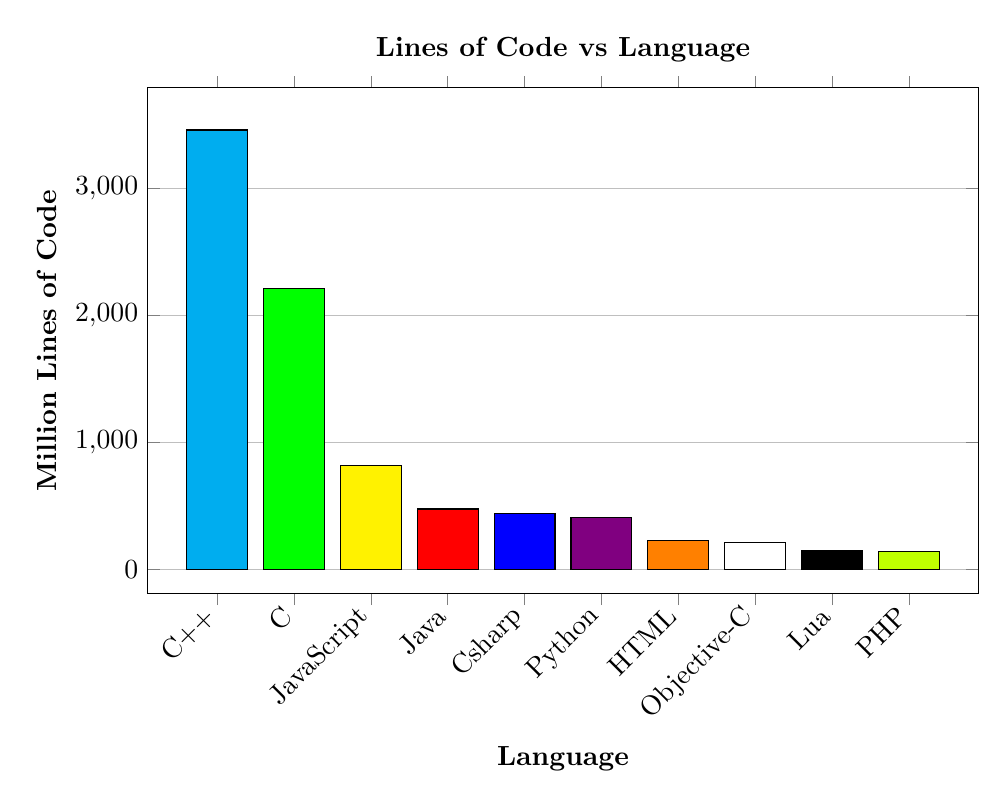
\begin{tikzpicture}
    \begin{axis}[
            title style={font=\bfseries},
            title={Lines of Code vs Language},
            label style={font=\bfseries},
            ylabel={Million Lines of Code},
            xlabel={Language},
            ybar=0pt,
            bar shift=0pt,
            width=\textwidth,
            height=8cm,
            bar width=22pt,
            ymajorgrids,
            xticklabel style={rotate=45, anchor=east},
            symbolic x coords={C++,C,JavaScript,Java,Csharp,Python, HTML,Objective-C,Lua,PHP},
        ]
        \addplot[fill=cyan]     coordinates {(C++,           3458.479714)};
        \addplot[fill=green]    coordinates {(C,             2209.641322)};
        \addplot[fill=yellow]   coordinates {(JavaScript,    817.837288)};
        \addplot[fill=red]      coordinates {(Java,          476.130697)};
        \addplot[fill=blue]     coordinates {(Csharp,        442.194502)};
        \addplot[fill=violet]   coordinates {(Python,        410.332101)};
        \addplot[fill=orange]   coordinates {(HTML,          225.246790)};
        \addplot[fill=white]    coordinates {(Objective-C,   210.542192)};
        \addplot[fill=black]    coordinates {(Lua,           149.334261)};
        \addplot[fill=lime]     coordinates {(PHP,           144.423927)};
    \end{axis}
\end{tikzpicture}
\caption{Lines of code of top 10 languages}
\label{fig:loc-top10} 
\end{figure}

These findings are mostly in line with a survey of game development ads posted on Gamasutra.com \cite{gamasutra:mostUsedProgrammingLanguage}. Here the top four languages in game development jobs are C++, C\#, Java and Lua. The high position of Lua could be caused by the closer connection to game development industry or the sample size of 46 ads.
